\section{RESULTS}
    The following results were obtained simulating with ticks 1500, with initial healthy (71), risky (10) and diabetic (29).
    
    The results are presented in \cref{fig:res}. In the simulation, initially, agents delay changing their marital status, however, when they start marrying, social pressure starts increasing and, consequently, they begin marrying more often. Additionally, as marriages have an incidence on the BMI level, it must increase as well. Similarly, the number of diabetic individuals has to increase, since the BMI influence it with certain probabilities. This fact directly implies that the number of risky and healthy individuals need to decrease.
 
    \begin{figure}
        \centering
        \begin{subfigure}[b]{0.3\columnwidth}
            \centering
            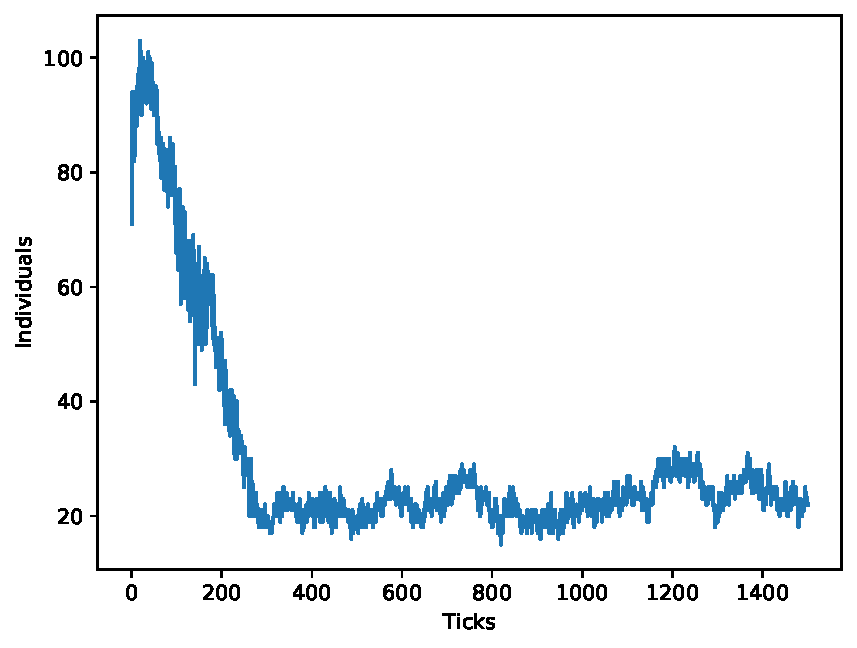
\includegraphics[width=1\columnwidth]{files/results-healthy.pdf}
            \caption{Healthy.}
            \label{subfig:control}
        \end{subfigure} 
        \begin{subfigure}[b]{0.3\columnwidth}
            \centering 
            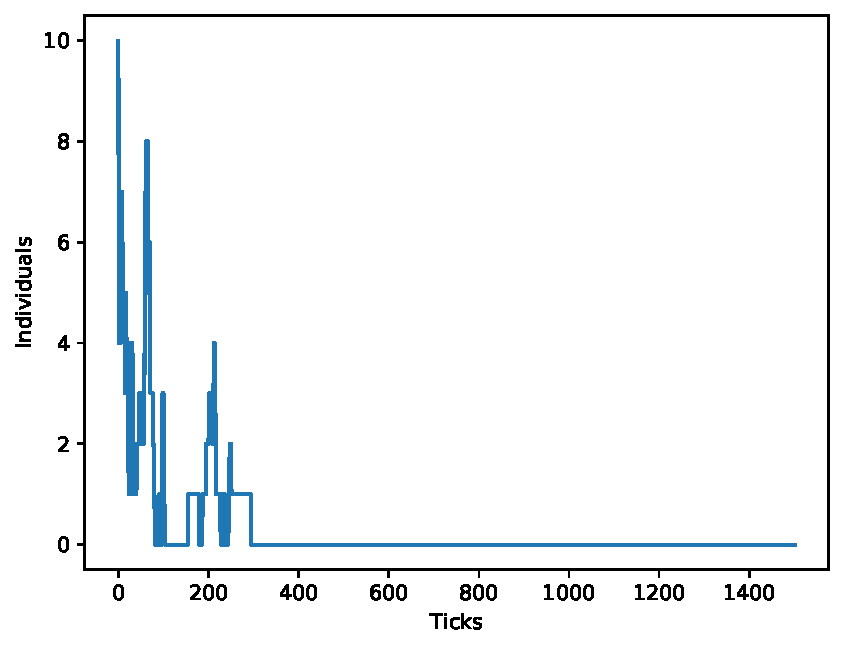
\includegraphics[width=1\columnwidth]{files/results-risk.pdf}
            \caption{Risky.}
            \label{subfig:sol}
        \end{subfigure}
        \begin{subfigure}[b]{0.3\columnwidth}
            \centering 
            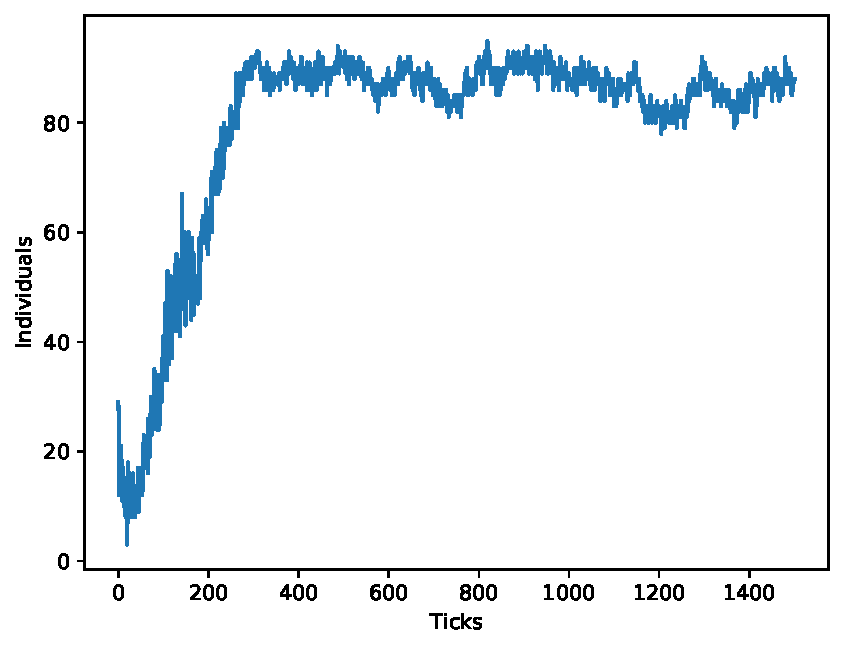
\includegraphics[width=1\columnwidth]{files/results-diabetes.pdf}
            \caption{Diabetic.}
            \label{subfig:sol}
        \end{subfigure}\\
        \begin{subfigure}[b]{0.3\columnwidth}
            \centering 
            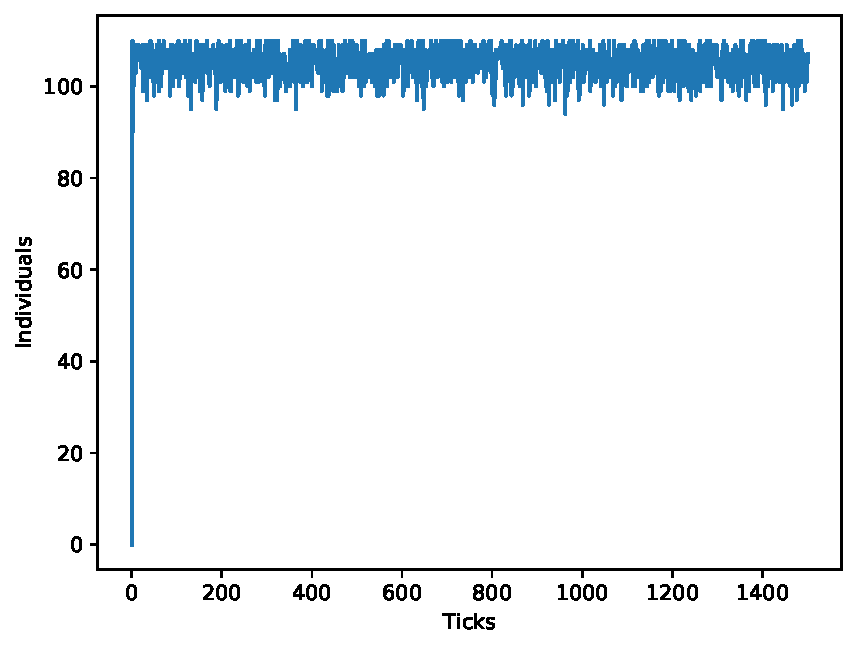
\includegraphics[width=1\columnwidth]{files/results-married.pdf}
            \caption{Married agents.}
            \label{subfig:sol}
        \end{subfigure}
        \begin{subfigure}[b]{0.3\columnwidth}
            \centering 
            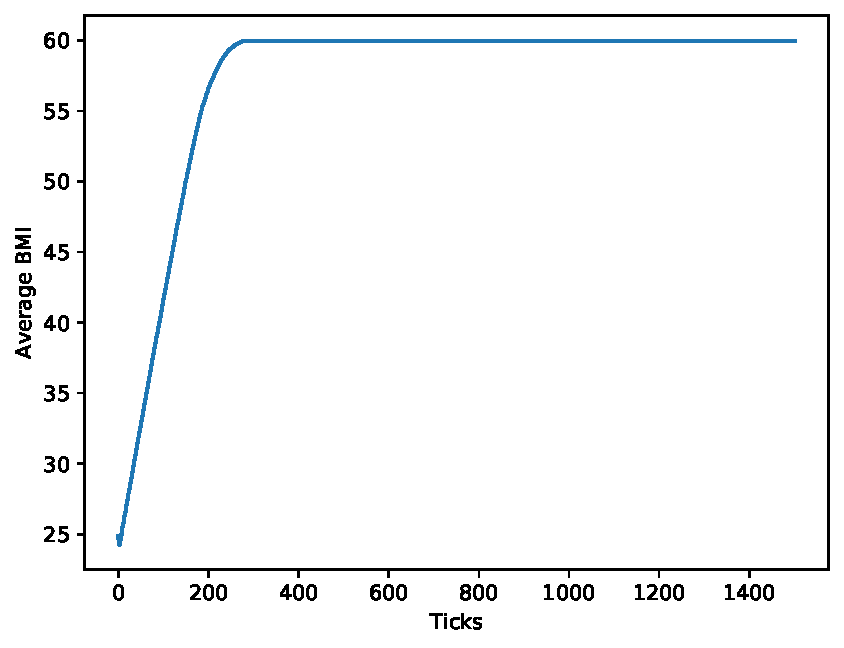
\includegraphics[width=1\columnwidth]{files/results-bmi.pdf}
            \caption{Average BMI.}
            \label{subfig:sol}
        \end{subfigure}
        \caption{Results for one diabetic individual.}
        \label{fig:res}
	\end{figure}
